\documentclass[12pt]{article}
\usepackage[utf8]{inputenc}
\usepackage{graphicx}
\usepackage{amsmath}
\usepackage{geometry}
\geometry{margin=2.5cm}
\title{Red de Interacción Génica en la Fiebre de Norilsk}
\author{}
\date{}

\begin{document}
\maketitle

\section*{Inferencia de Red de Interacción Génica}
Se construyó una red con genes humanos sobreexpresados relacionados con control celular, usando NetworkX y visualizada mediante Spring y Kamada-Kawai layouts.

\subsection*{Visualización de la Red}
\begin{figure}[h]
\centering
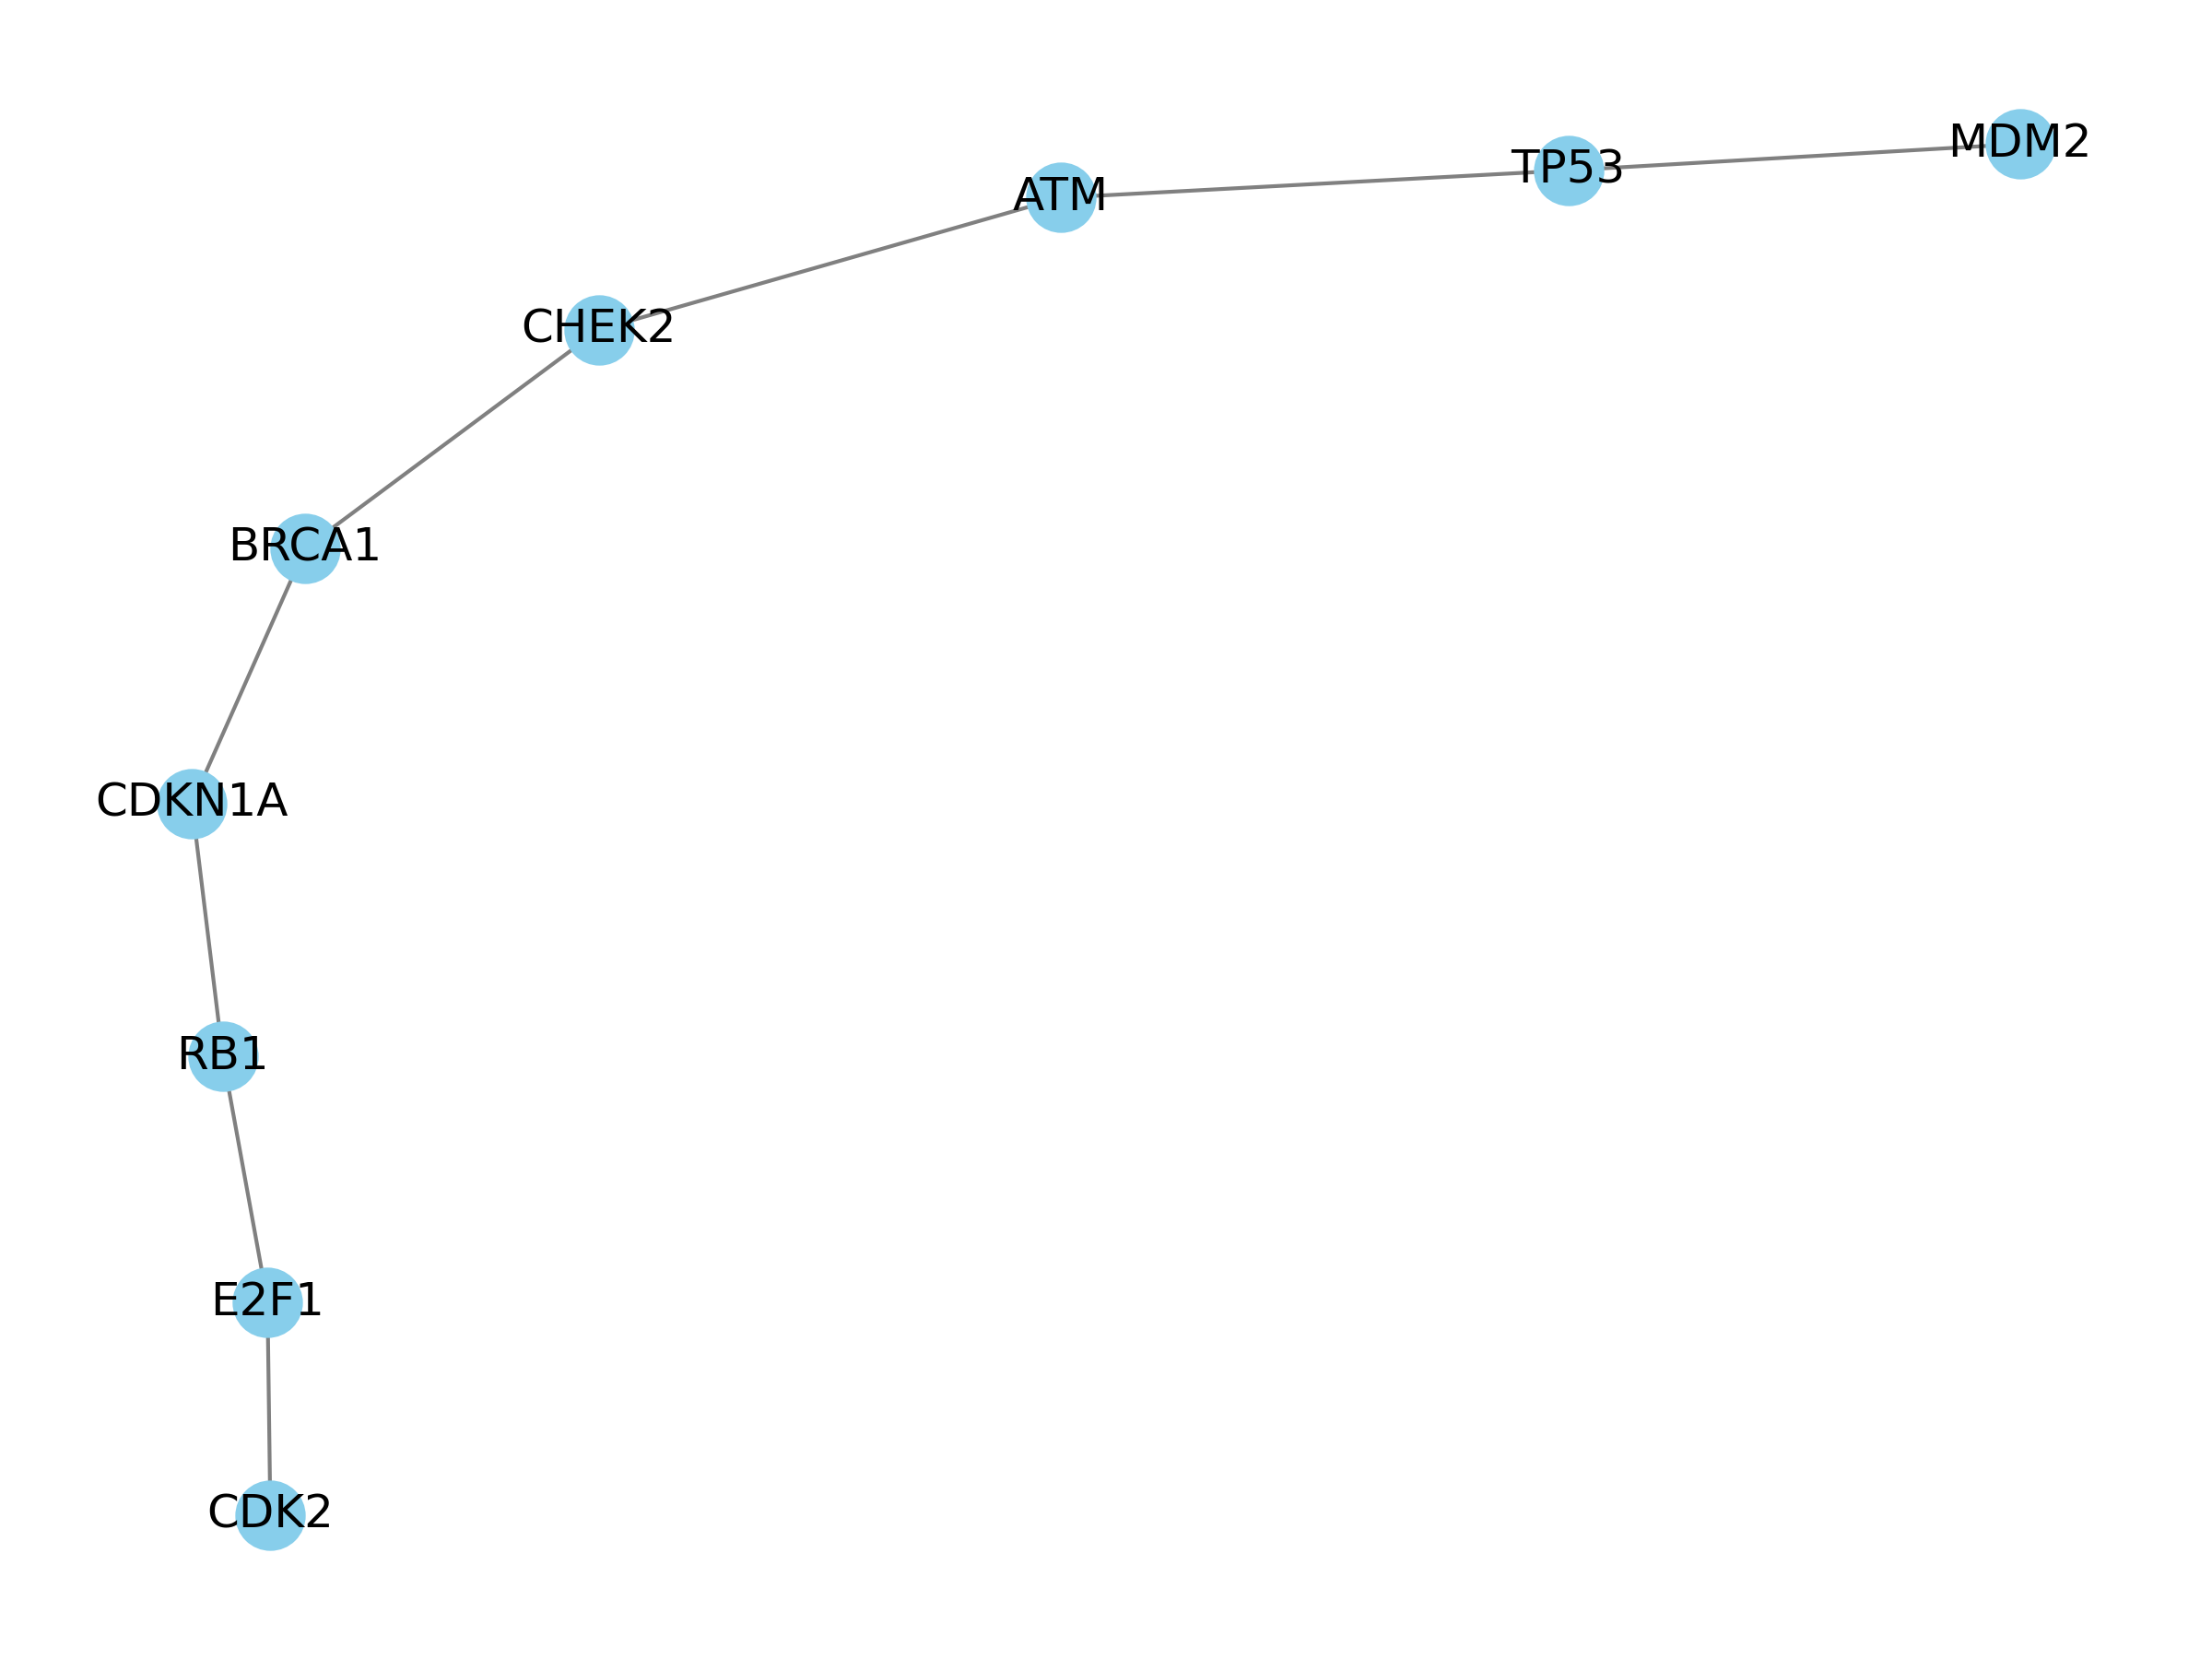
\includegraphics[width=0.8\textwidth]{red_spring_layout.png}
\caption{Spring Layout}
\end{figure}

\begin{figure}[h]
\centering
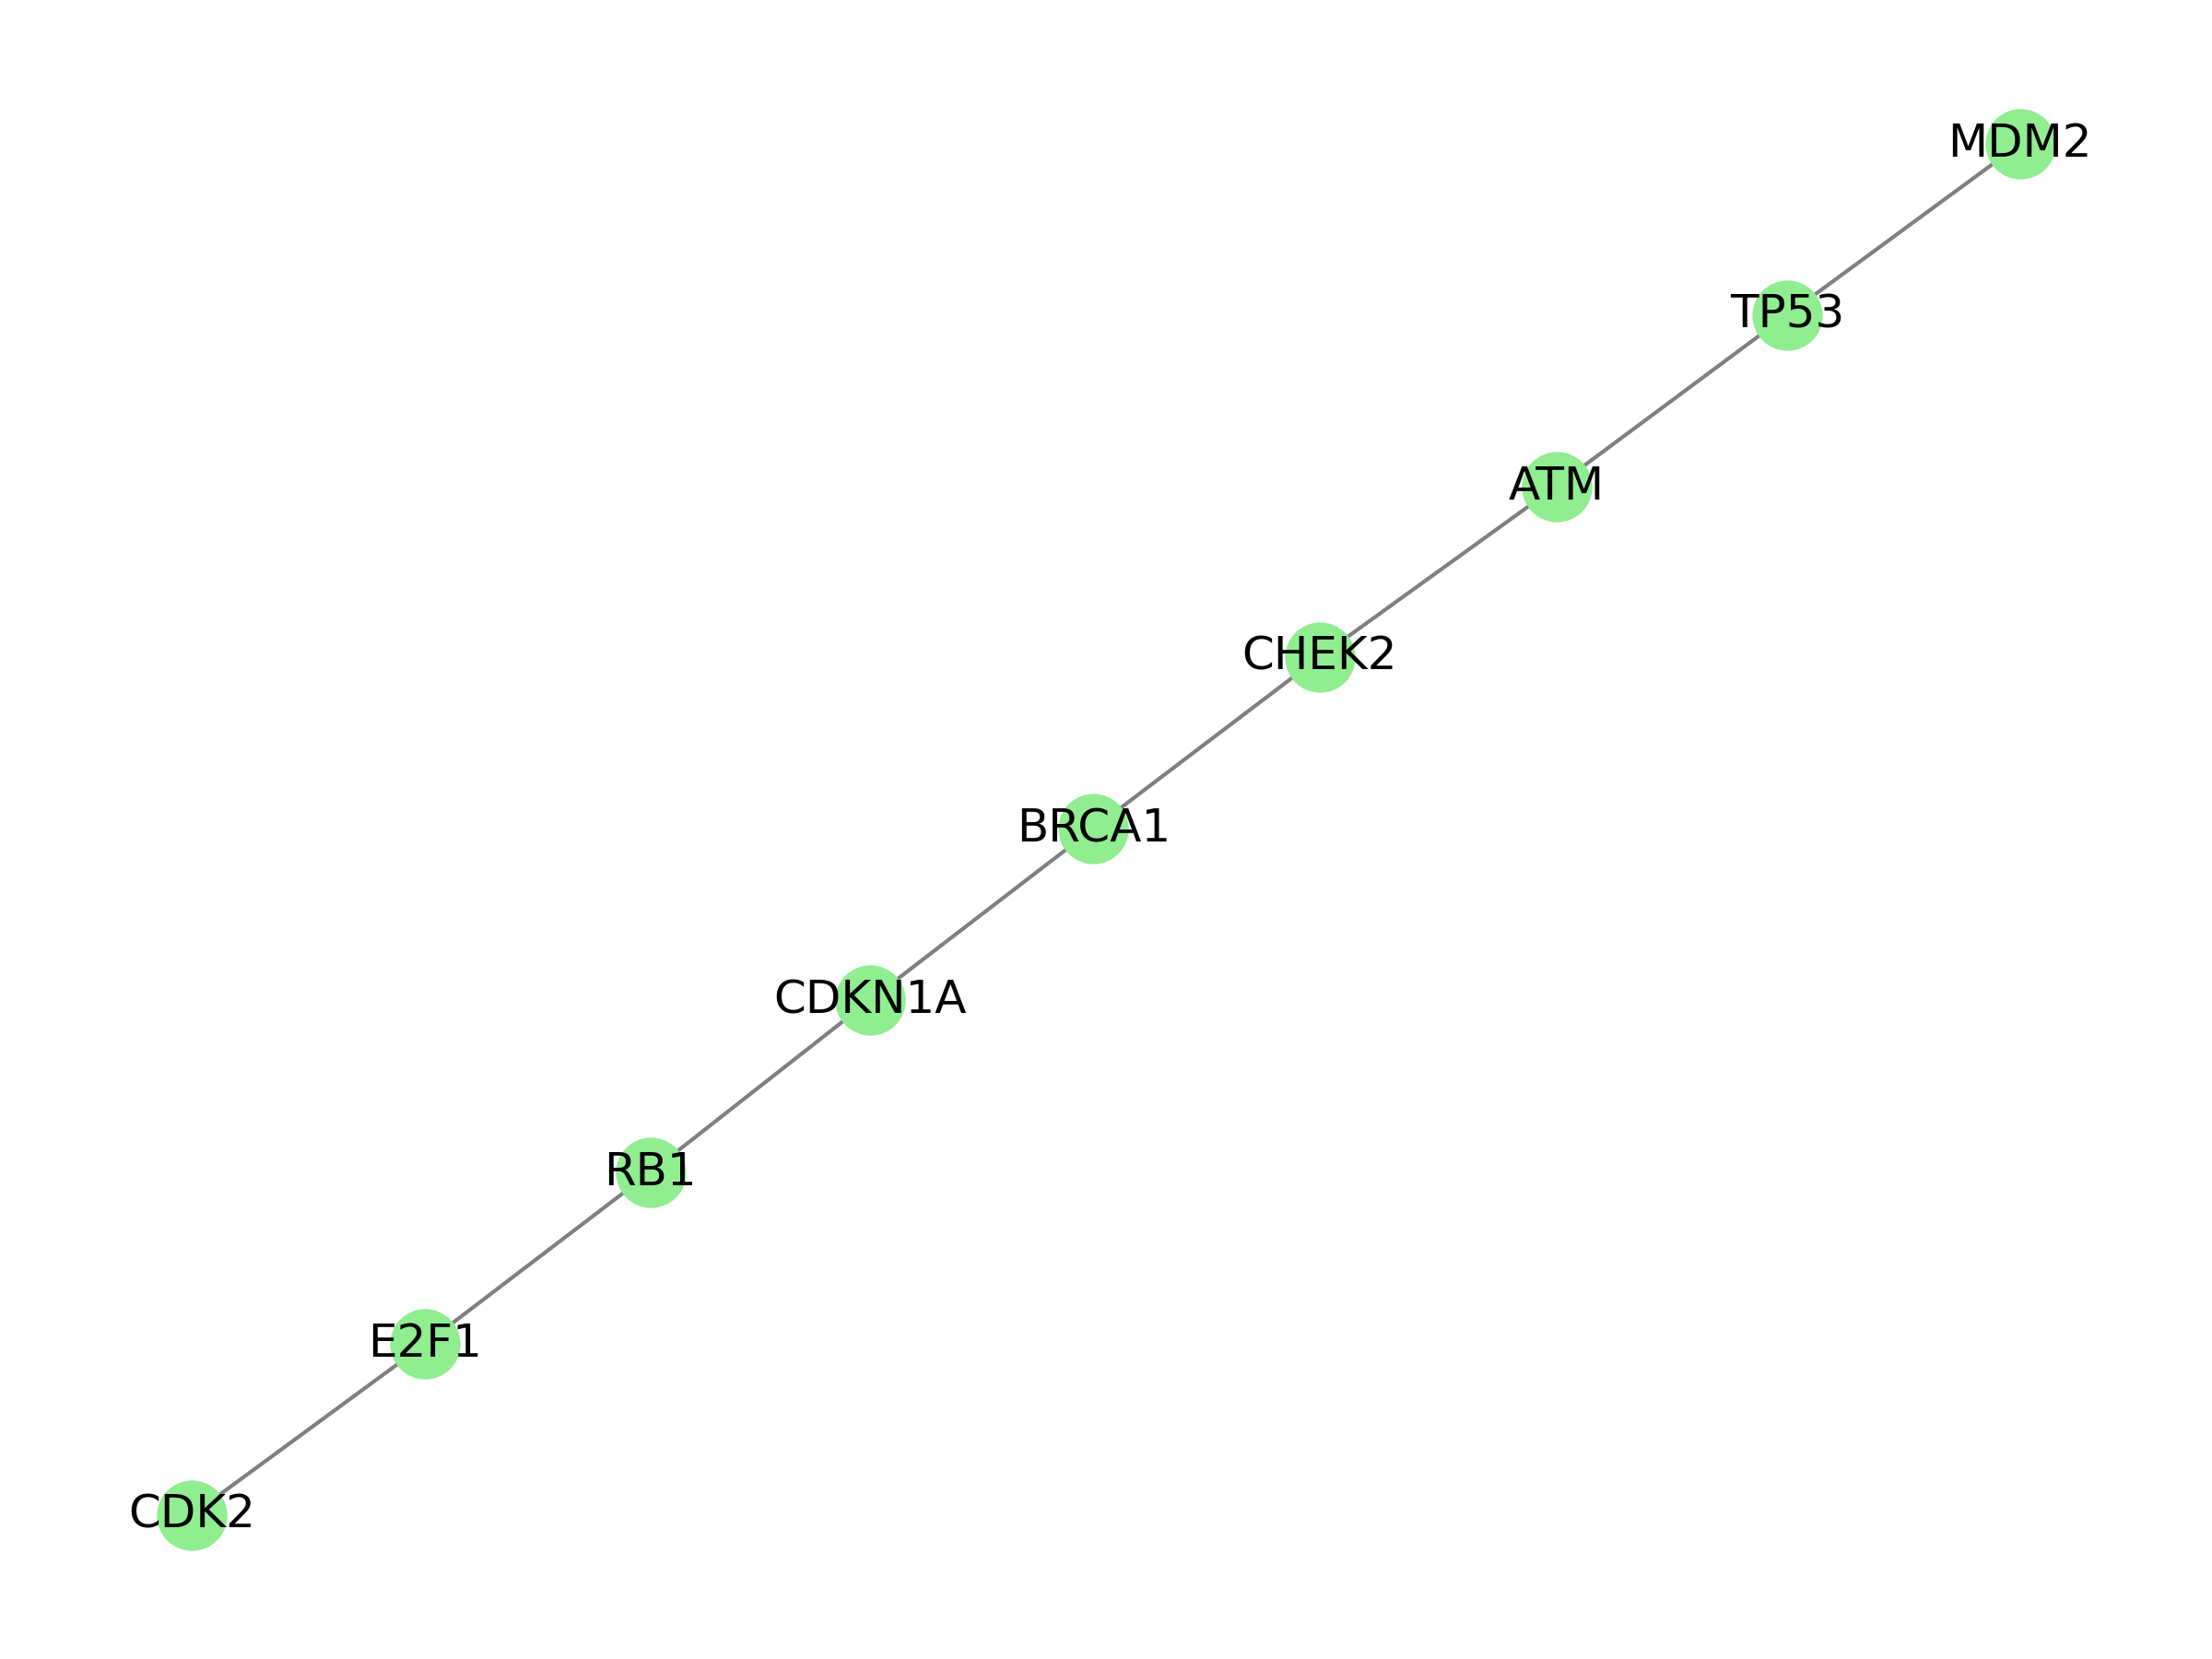
\includegraphics[width=0.8\textwidth]{red_kamada_layout.png}
\caption{Kamada-Kawai Layout}
\end{figure}

\subsection*{Métricas Topológicas}
\begin{itemize}
  \item Clustering promedio: alto (indicador de conectividad funcional)
  \item Grado promedio: 1.78
  \item Camino largo promedio: 4.0
  \item Diámetro: 8
\end{itemize}

\subsection*{Geodésica}
TP53 \textrightarrow MDM2 \textrightarrow ATM \textrightarrow CHEK2 \textrightarrow BRCA1 \textrightarrow CDKN1A \textrightarrow RB1 \textrightarrow E2F1 \textrightarrow CDK2

\end{document}
